\documentclass[twoside]{book}

% Packages required by doxygen
\usepackage{fixltx2e}
\usepackage{calc}
\usepackage{doxygen}
\usepackage[export]{adjustbox} % also loads graphicx
\usepackage{graphicx}
\usepackage[utf8]{inputenc}
\usepackage{makeidx}
\usepackage{multicol}
\usepackage{multirow}
\PassOptionsToPackage{warn}{textcomp}
\usepackage{textcomp}
\usepackage[nointegrals]{wasysym}
\usepackage[table]{xcolor}

% Font selection
\usepackage[T1]{fontenc}
\usepackage[scaled=.90]{helvet}
\usepackage{courier}
\usepackage{amssymb}
\usepackage{sectsty}
\renewcommand{\familydefault}{\sfdefault}
\allsectionsfont{%
  \fontseries{bc}\selectfont%
  \color{darkgray}%
}
\renewcommand{\DoxyLabelFont}{%
  \fontseries{bc}\selectfont%
  \color{darkgray}%
}
\newcommand{\+}{\discretionary{\mbox{\scriptsize$\hookleftarrow$}}{}{}}

% Page & text layout
\usepackage{geometry}
\geometry{%
  a4paper,%
  top=2.5cm,%
  bottom=2.5cm,%
  left=2.5cm,%
  right=2.5cm%
}
\tolerance=750
\hfuzz=15pt
\hbadness=750
\setlength{\emergencystretch}{15pt}
\setlength{\parindent}{0cm}
\setlength{\parskip}{3ex plus 2ex minus 2ex}
\makeatletter
\renewcommand{\paragraph}{%
  \@startsection{paragraph}{4}{0ex}{-1.0ex}{1.0ex}{%
    \normalfont\normalsize\bfseries\SS@parafont%
  }%
}
\renewcommand{\subparagraph}{%
  \@startsection{subparagraph}{5}{0ex}{-1.0ex}{1.0ex}{%
    \normalfont\normalsize\bfseries\SS@subparafont%
  }%
}
\makeatother

% Headers & footers
\usepackage{fancyhdr}
\pagestyle{fancyplain}
\fancyhead[LE]{\fancyplain{}{\bfseries\thepage}}
\fancyhead[CE]{\fancyplain{}{}}
\fancyhead[RE]{\fancyplain{}{\bfseries\leftmark}}
\fancyhead[LO]{\fancyplain{}{\bfseries\rightmark}}
\fancyhead[CO]{\fancyplain{}{}}
\fancyhead[RO]{\fancyplain{}{\bfseries\thepage}}
\fancyfoot[LE]{\fancyplain{}{}}
\fancyfoot[CE]{\fancyplain{}{}}
\fancyfoot[RE]{\fancyplain{}{\bfseries\scriptsize Generated by Doxygen }}
\fancyfoot[LO]{\fancyplain{}{\bfseries\scriptsize Generated by Doxygen }}
\fancyfoot[CO]{\fancyplain{}{}}
\fancyfoot[RO]{\fancyplain{}{}}
\renewcommand{\footrulewidth}{0.4pt}
\renewcommand{\chaptermark}[1]{%
  \markboth{#1}{}%
}
\renewcommand{\sectionmark}[1]{%
  \markright{\thesection\ #1}%
}

% Indices & bibliography
\usepackage{natbib}
\usepackage[titles]{tocloft}
\setcounter{tocdepth}{3}
\setcounter{secnumdepth}{5}
\makeindex

% Hyperlinks (required, but should be loaded last)
\usepackage{ifpdf}
\ifpdf
  \usepackage[pdftex,pagebackref=true]{hyperref}
\else
  \usepackage[ps2pdf,pagebackref=true]{hyperref}
\fi
\hypersetup{%
  colorlinks=true,%
  linkcolor=blue,%
  citecolor=blue,%
  unicode%
}

% Custom commands
\newcommand{\clearemptydoublepage}{%
  \newpage{\pagestyle{empty}\cleardoublepage}%
}

\usepackage{caption}
\captionsetup{labelsep=space,justification=centering,font={bf},singlelinecheck=off,skip=4pt,position=top}

%===== C O N T E N T S =====

\begin{document}

% Titlepage & ToC
\hypersetup{pageanchor=false,
             bookmarksnumbered=true,
             pdfencoding=unicode
            }
\pagenumbering{roman}
\begin{titlepage}
\vspace*{7cm}
\begin{center}%
{\Large My Project }\\
\vspace*{1cm}
{\large Generated by Doxygen 1.8.11}\\
\end{center}
\end{titlepage}
\clearemptydoublepage
\tableofcontents
\clearemptydoublepage
\pagenumbering{arabic}
\hypersetup{pageanchor=true}

%--- Begin generated contents ---
\chapter{Class Index}
\section{Class List}
Here are the classes, structs, unions and interfaces with brief descriptions\+:\begin{DoxyCompactList}
\item\contentsline{section}{\hyperlink{structnode}{node} }{\pageref{structnode}}{}
\item\contentsline{section}{\hyperlink{structnode1}{node1} }{\pageref{structnode1}}{}
\item\contentsline{section}{\hyperlink{structnode__info}{node\+\_\+info} }{\pageref{structnode__info}}{}
\end{DoxyCompactList}

\chapter{File Index}
\section{File List}
Here is a list of all files with brief descriptions\+:\begin{DoxyCompactList}
\item\contentsline{section}{\hyperlink{Lab1_8c}{Lab1.\+c} }{\pageref{Lab1_8c}}{}
\end{DoxyCompactList}

\chapter{Class Documentation}
\hypertarget{classPoint}{}\section{Point Class Reference}
\label{classPoint}\index{Point@{Point}}


{\ttfamily \#include $<$Point.\+h$>$}

\subsection*{Public Member Functions}
\begin{DoxyCompactItemize}
\item 
\hyperlink{classPoint_a1c8a6881ed0f11828299033c5959d147}{Point} (int \hyperlink{classPoint_a8c779e11e694b20e0946105a9f5de842}{x}=0, int \hyperlink{classPoint_a2e1b5fb2b2a83571f5c0bc0f66a73cf7}{y}=0)
\item 
int \hyperlink{classPoint_abe622fffc8785b0c2e06cdac681b9837}{getX} () const 
\item 
void \hyperlink{classPoint_acdc86ab607b2ae8415152883e2629015}{setX} (int \hyperlink{classPoint_a8c779e11e694b20e0946105a9f5de842}{x})
\item 
int \hyperlink{classPoint_a10f31e48e2dbc22e3660ca769b8d5d65}{getY} () const 
\item 
void \hyperlink{classPoint_afccad787a359f062efc1af5e935a99ba}{setY} (int \hyperlink{classPoint_a2e1b5fb2b2a83571f5c0bc0f66a73cf7}{y})
\item 
void \hyperlink{classPoint_afb6a0c9ad81c0864e4039069f0f33d80}{set\+XY} (int \hyperlink{classPoint_a8c779e11e694b20e0946105a9f5de842}{x}, int \hyperlink{classPoint_a2e1b5fb2b2a83571f5c0bc0f66a73cf7}{y})
\item 
double \hyperlink{classPoint_a96a23567344de8c84468a96f97c2448f}{get\+Magnitude} () const 
\item 
double \hyperlink{classPoint_ae53cf4bc004996960585a70948a21cb6}{get\+Argument} () const 
\item 
void \hyperlink{classPoint_a20b27dff6a871012fa5e7c0d52fd6b98}{print} () const 
\end{DoxyCompactItemize}
\subsection*{Private Attributes}
\begin{DoxyCompactItemize}
\item 
int \hyperlink{classPoint_a8c779e11e694b20e0946105a9f5de842}{x}
\item 
int \hyperlink{classPoint_a2e1b5fb2b2a83571f5c0bc0f66a73cf7}{y}
\end{DoxyCompactItemize}


\subsection{Constructor \& Destructor Documentation}
\index{Point@{Point}!Point@{Point}}
\index{Point@{Point}!Point@{Point}}
\subsubsection[{\texorpdfstring{Point(int x=0, int y=0)}{Point(int x=0, int y=0)}}]{\setlength{\rightskip}{0pt plus 5cm}Point\+::\+Point (
\begin{DoxyParamCaption}
\item[{int}]{x = {\ttfamily 0}, }
\item[{int}]{y = {\ttfamily 0}}
\end{DoxyParamCaption}
)}\hypertarget{classPoint_a1c8a6881ed0f11828299033c5959d147}{}\label{classPoint_a1c8a6881ed0f11828299033c5959d147}

\begin{DoxyCode}
8 : \hyperlink{classPoint_a8c779e11e694b20e0946105a9f5de842}{x}(\hyperlink{classPoint_a8c779e11e694b20e0946105a9f5de842}{x}), \hyperlink{classPoint_a2e1b5fb2b2a83571f5c0bc0f66a73cf7}{y}(\hyperlink{classPoint_a2e1b5fb2b2a83571f5c0bc0f66a73cf7}{y}) \{ \}  \textcolor{comment}{// Use member initializer list}
\end{DoxyCode}


\subsection{Member Function Documentation}
\index{Point@{Point}!get\+Argument@{get\+Argument}}
\index{get\+Argument@{get\+Argument}!Point@{Point}}
\subsubsection[{\texorpdfstring{get\+Argument() const }{getArgument() const }}]{\setlength{\rightskip}{0pt plus 5cm}double Point\+::get\+Argument (
\begin{DoxyParamCaption}
{}
\end{DoxyParamCaption}
) const}\hypertarget{classPoint_ae53cf4bc004996960585a70948a21cb6}{}\label{classPoint_ae53cf4bc004996960585a70948a21cb6}

\begin{DoxyCode}
42                                 \{
43    \textcolor{keywordflow}{return} atan2(\hyperlink{classPoint_a2e1b5fb2b2a83571f5c0bc0f66a73cf7}{y}, \hyperlink{classPoint_a8c779e11e694b20e0946105a9f5de842}{x});    \textcolor{comment}{// atan2 in <cmath>}
44 \}
\end{DoxyCode}
\index{Point@{Point}!get\+Magnitude@{get\+Magnitude}}
\index{get\+Magnitude@{get\+Magnitude}!Point@{Point}}
\subsubsection[{\texorpdfstring{get\+Magnitude() const }{getMagnitude() const }}]{\setlength{\rightskip}{0pt plus 5cm}double Point\+::get\+Magnitude (
\begin{DoxyParamCaption}
{}
\end{DoxyParamCaption}
) const}\hypertarget{classPoint_a96a23567344de8c84468a96f97c2448f}{}\label{classPoint_a96a23567344de8c84468a96f97c2448f}

\begin{DoxyCode}
37                                  \{
38    \textcolor{keywordflow}{return} sqrt(\hyperlink{classPoint_a8c779e11e694b20e0946105a9f5de842}{x}*\hyperlink{classPoint_a8c779e11e694b20e0946105a9f5de842}{x} + \hyperlink{classPoint_a2e1b5fb2b2a83571f5c0bc0f66a73cf7}{y}*\hyperlink{classPoint_a2e1b5fb2b2a83571f5c0bc0f66a73cf7}{y});    \textcolor{comment}{// sqrt in <cmath>}
39 \}
\end{DoxyCode}
\index{Point@{Point}!getX@{getX}}
\index{getX@{getX}!Point@{Point}}
\subsubsection[{\texorpdfstring{get\+X() const }{getX() const }}]{\setlength{\rightskip}{0pt plus 5cm}int Point\+::getX (
\begin{DoxyParamCaption}
{}
\end{DoxyParamCaption}
) const}\hypertarget{classPoint_abe622fffc8785b0c2e06cdac681b9837}{}\label{classPoint_abe622fffc8785b0c2e06cdac681b9837}

\begin{DoxyCode}
11                       \{
12    \textcolor{keywordflow}{return} \hyperlink{classPoint_a8c779e11e694b20e0946105a9f5de842}{x};
13 \}
\end{DoxyCode}
\index{Point@{Point}!getY@{getY}}
\index{getY@{getY}!Point@{Point}}
\subsubsection[{\texorpdfstring{get\+Y() const }{getY() const }}]{\setlength{\rightskip}{0pt plus 5cm}int Point\+::getY (
\begin{DoxyParamCaption}
{}
\end{DoxyParamCaption}
) const}\hypertarget{classPoint_a10f31e48e2dbc22e3660ca769b8d5d65}{}\label{classPoint_a10f31e48e2dbc22e3660ca769b8d5d65}

\begin{DoxyCode}
21                       \{
22    \textcolor{keywordflow}{return} \hyperlink{classPoint_a2e1b5fb2b2a83571f5c0bc0f66a73cf7}{y};
23 \}
\end{DoxyCode}
\index{Point@{Point}!print@{print}}
\index{print@{print}!Point@{Point}}
\subsubsection[{\texorpdfstring{print() const }{print() const }}]{\setlength{\rightskip}{0pt plus 5cm}void Point\+::print (
\begin{DoxyParamCaption}
{}
\end{DoxyParamCaption}
) const}\hypertarget{classPoint_a20b27dff6a871012fa5e7c0d52fd6b98}{}\label{classPoint_a20b27dff6a871012fa5e7c0d52fd6b98}

\begin{DoxyCode}
47                         \{
48    cout << \textcolor{stringliteral}{"("} << \hyperlink{classPoint_a8c779e11e694b20e0946105a9f5de842}{x} << \textcolor{stringliteral}{","} << \hyperlink{classPoint_a2e1b5fb2b2a83571f5c0bc0f66a73cf7}{y} << \textcolor{stringliteral}{")"} << endl;
49 \}\end{DoxyCode}
\index{Point@{Point}!setX@{setX}}
\index{setX@{setX}!Point@{Point}}
\subsubsection[{\texorpdfstring{set\+X(int x)}{setX(int x)}}]{\setlength{\rightskip}{0pt plus 5cm}void Point\+::setX (
\begin{DoxyParamCaption}
\item[{int}]{x}
\end{DoxyParamCaption}
)}\hypertarget{classPoint_acdc86ab607b2ae8415152883e2629015}{}\label{classPoint_acdc86ab607b2ae8415152883e2629015}

\begin{DoxyCode}
16                       \{
17    this->\hyperlink{classPoint_a8c779e11e694b20e0946105a9f5de842}{x} = \hyperlink{classPoint_a8c779e11e694b20e0946105a9f5de842}{x};
18 \}
\end{DoxyCode}
\index{Point@{Point}!set\+XY@{set\+XY}}
\index{set\+XY@{set\+XY}!Point@{Point}}
\subsubsection[{\texorpdfstring{set\+X\+Y(int x, int y)}{setXY(int x, int y)}}]{\setlength{\rightskip}{0pt plus 5cm}void Point\+::set\+XY (
\begin{DoxyParamCaption}
\item[{int}]{x, }
\item[{int}]{y}
\end{DoxyParamCaption}
)}\hypertarget{classPoint_afb6a0c9ad81c0864e4039069f0f33d80}{}\label{classPoint_afb6a0c9ad81c0864e4039069f0f33d80}

\begin{DoxyCode}
31                               \{
32    \hyperlink{classPoint_acdc86ab607b2ae8415152883e2629015}{setX}(\hyperlink{classPoint_a8c779e11e694b20e0946105a9f5de842}{x});
33    \hyperlink{classPoint_afccad787a359f062efc1af5e935a99ba}{setY}(\hyperlink{classPoint_a2e1b5fb2b2a83571f5c0bc0f66a73cf7}{y});
34 \}
\end{DoxyCode}


Here is the call graph for this function\+:
\nopagebreak
\begin{figure}[H]
\begin{center}
\leavevmode
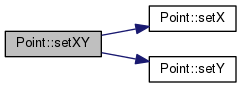
\includegraphics[width=253pt]{classPoint_afb6a0c9ad81c0864e4039069f0f33d80_cgraph}
\end{center}
\end{figure}


\index{Point@{Point}!setY@{setY}}
\index{setY@{setY}!Point@{Point}}
\subsubsection[{\texorpdfstring{set\+Y(int y)}{setY(int y)}}]{\setlength{\rightskip}{0pt plus 5cm}void Point\+::setY (
\begin{DoxyParamCaption}
\item[{int}]{y}
\end{DoxyParamCaption}
)}\hypertarget{classPoint_afccad787a359f062efc1af5e935a99ba}{}\label{classPoint_afccad787a359f062efc1af5e935a99ba}

\begin{DoxyCode}
26                       \{
27    this->\hyperlink{classPoint_a2e1b5fb2b2a83571f5c0bc0f66a73cf7}{y} = \hyperlink{classPoint_a2e1b5fb2b2a83571f5c0bc0f66a73cf7}{y};
28 \}
\end{DoxyCode}


\subsection{Member Data Documentation}
\index{Point@{Point}!x@{x}}
\index{x@{x}!Point@{Point}}
\subsubsection[{\texorpdfstring{x}{x}}]{\setlength{\rightskip}{0pt plus 5cm}int Point\+::x\hspace{0.3cm}{\ttfamily [private]}}\hypertarget{classPoint_a8c779e11e694b20e0946105a9f5de842}{}\label{classPoint_a8c779e11e694b20e0946105a9f5de842}
\index{Point@{Point}!y@{y}}
\index{y@{y}!Point@{Point}}
\subsubsection[{\texorpdfstring{y}{y}}]{\setlength{\rightskip}{0pt plus 5cm}int Point\+::y\hspace{0.3cm}{\ttfamily [private]}}\hypertarget{classPoint_a2e1b5fb2b2a83571f5c0bc0f66a73cf7}{}\label{classPoint_a2e1b5fb2b2a83571f5c0bc0f66a73cf7}


The documentation for this class was generated from the following files\+:\begin{DoxyCompactItemize}
\item 
\hyperlink{Point_8h}{Point.\+h}\item 
\hyperlink{Point_8cpp}{Point.\+cpp}\end{DoxyCompactItemize}

\hypertarget{classPolygon}{}\section{Polygon Class Reference}
\label{classPolygon}\index{Polygon@{Polygon}}


Collaboration diagram for Polygon\+:
\nopagebreak
\begin{figure}[H]
\begin{center}
\leavevmode
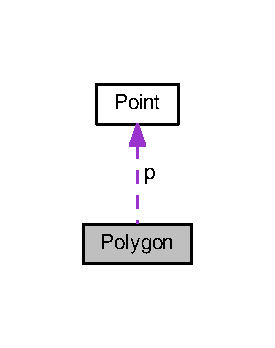
\includegraphics[width=132pt]{classPolygon__coll__graph}
\end{center}
\end{figure}
\subsection*{Public Member Functions}
\begin{DoxyCompactItemize}
\item 
\hyperlink{classPolygon_ac183e712f8be1e13f1c9d5b4d4512ead}{Polygon} ()
\end{DoxyCompactItemize}
\subsection*{Public Attributes}
\begin{DoxyCompactItemize}
\item 
\hyperlink{classPoint}{Point} \hyperlink{classPolygon_ab9eed6eb2dc3e7e51e8b88e144bf68d0}{p} \mbox{[}\hyperlink{Slicker_8cpp_ae936b8f2104cec7519d956be29b10e2b}{M\+A\+X\+P\+O\+LY}\mbox{]}
\item 
int \hyperlink{classPolygon_a96568fe72cac8ee98d09cf62fd24a8ed}{n}
\end{DoxyCompactItemize}


\subsection{Constructor \& Destructor Documentation}
\index{Polygon@{Polygon}!Polygon@{Polygon}}
\index{Polygon@{Polygon}!Polygon@{Polygon}}
\subsubsection[{\texorpdfstring{Polygon()}{Polygon()}}]{\setlength{\rightskip}{0pt plus 5cm}Polygon\+::\+Polygon (
\begin{DoxyParamCaption}
{}
\end{DoxyParamCaption}
)\hspace{0.3cm}{\ttfamily [inline]}}\hypertarget{classPolygon_ac183e712f8be1e13f1c9d5b4d4512ead}{}\label{classPolygon_ac183e712f8be1e13f1c9d5b4d4512ead}

\begin{DoxyCode}
23         \{
24             \textcolor{keywordflow}{for} (\textcolor{keywordtype}{int} i = 0; i < \hyperlink{Slicker_8cpp_ae936b8f2104cec7519d956be29b10e2b}{MAXPOLY}; i++)
25                 \hyperlink{classPoint}{Point} \hyperlink{classPolygon_ab9eed6eb2dc3e7e51e8b88e144bf68d0}{p}[i];\textcolor{comment}{// = new Point();}
26         \}
\end{DoxyCode}


\subsection{Member Data Documentation}
\index{Polygon@{Polygon}!n@{n}}
\index{n@{n}!Polygon@{Polygon}}
\subsubsection[{\texorpdfstring{n}{n}}]{\setlength{\rightskip}{0pt plus 5cm}int Polygon\+::n}\hypertarget{classPolygon_a96568fe72cac8ee98d09cf62fd24a8ed}{}\label{classPolygon_a96568fe72cac8ee98d09cf62fd24a8ed}
\index{Polygon@{Polygon}!p@{p}}
\index{p@{p}!Polygon@{Polygon}}
\subsubsection[{\texorpdfstring{p}{p}}]{\setlength{\rightskip}{0pt plus 5cm}{\bf Point} Polygon\+::p\mbox{[}{\bf M\+A\+X\+P\+O\+LY}\mbox{]}}\hypertarget{classPolygon_ab9eed6eb2dc3e7e51e8b88e144bf68d0}{}\label{classPolygon_ab9eed6eb2dc3e7e51e8b88e144bf68d0}


The documentation for this class was generated from the following file\+:\begin{DoxyCompactItemize}
\item 
\hyperlink{Slicker_8cpp}{Slicker.\+cpp}\end{DoxyCompactItemize}

\chapter{File Documentation}
\hypertarget{Slicker_8cpp}{}\section{Slicker.\+cpp File Reference}
\label{Slicker_8cpp}\index{Slicker.\+cpp@{Slicker.\+cpp}}
{\ttfamily \#include $<$iostream$>$}\\*
Include dependency graph for Slicker.\+cpp\+:
\nopagebreak
\begin{figure}[H]
\begin{center}
\leavevmode
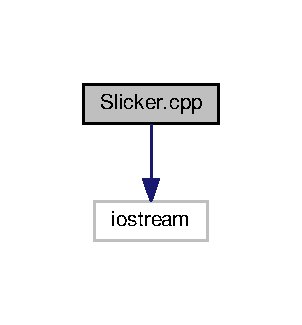
\includegraphics[width=145pt]{Slicker_8cpp__incl}
\end{center}
\end{figure}
\subsection*{Classes}
\begin{DoxyCompactItemize}
\item 
class \hyperlink{classPoint}{Point}
\item 
class \hyperlink{classPolygon}{Polygon}
\end{DoxyCompactItemize}
\subsection*{Functions}
\begin{DoxyCompactItemize}
\item 
double \hyperlink{Slicker_8cpp_a81592f7bc6730396f21d9685d9879b28}{area} (\hyperlink{classPolygon}{Polygon} p)
\item 
int \hyperlink{Slicker_8cpp_a3c04138a5bfe5d72780bb7e82a18e627}{main} (int argc, char $\ast$$\ast$argv)
\end{DoxyCompactItemize}
\subsection*{Variables}
\begin{DoxyCompactItemize}
\item 
const int \hyperlink{Slicker_8cpp_ae936b8f2104cec7519d956be29b10e2b}{M\+A\+X\+P\+O\+LY} = 200
\item 
double \hyperlink{Slicker_8cpp_a3644fc584736c1c2e36037a085c416b9}{E\+P\+S\+I\+L\+ON} = 0.\+000001
\end{DoxyCompactItemize}


\subsection{Function Documentation}
\index{Slicker.\+cpp@{Slicker.\+cpp}!area@{area}}
\index{area@{area}!Slicker.\+cpp@{Slicker.\+cpp}}
\subsubsection[{\texorpdfstring{area(\+Polygon p)}{area(Polygon p)}}]{\setlength{\rightskip}{0pt plus 5cm}double area (
\begin{DoxyParamCaption}
\item[{{\bf Polygon}}]{p}
\end{DoxyParamCaption}
)}\hypertarget{Slicker_8cpp_a81592f7bc6730396f21d9685d9879b28}{}\label{Slicker_8cpp_a81592f7bc6730396f21d9685d9879b28}

\begin{DoxyCode}
30 \{
31     \textcolor{keywordtype}{double} total = 0;
32     \textcolor{keywordflow}{for} (\textcolor{keywordtype}{int} i = 0; i < p.\hyperlink{classPolygon_a96568fe72cac8ee98d09cf62fd24a8ed}{n}; i++)
33     \{
34         \textcolor{keywordtype}{int} j = (i + 1) % p.\hyperlink{classPolygon_a96568fe72cac8ee98d09cf62fd24a8ed}{n};
35         total += (p.\hyperlink{classPolygon_ab9eed6eb2dc3e7e51e8b88e144bf68d0}{p}[i].\hyperlink{classPoint_ab99c56589bc8ad5fa5071387110a5bc7}{x} * p.\hyperlink{classPolygon_ab9eed6eb2dc3e7e51e8b88e144bf68d0}{p}[j].\hyperlink{classPoint_afa38be143ae800e6ad69ce8ed4df62d8}{y}) - (p.\hyperlink{classPolygon_ab9eed6eb2dc3e7e51e8b88e144bf68d0}{p}[j].\hyperlink{classPoint_ab99c56589bc8ad5fa5071387110a5bc7}{x} * p.\hyperlink{classPolygon_ab9eed6eb2dc3e7e51e8b88e144bf68d0}{p}[i].\hyperlink{classPoint_afa38be143ae800e6ad69ce8ed4df62d8}{y});
36     \}
37     \textcolor{keywordflow}{return} total / 2;
38 \}
\end{DoxyCode}
\index{Slicker.\+cpp@{Slicker.\+cpp}!main@{main}}
\index{main@{main}!Slicker.\+cpp@{Slicker.\+cpp}}
\subsubsection[{\texorpdfstring{main(int argc, char $\ast$$\ast$argv)}{main(int argc, char **argv)}}]{\setlength{\rightskip}{0pt plus 5cm}int main (
\begin{DoxyParamCaption}
\item[{int}]{argc, }
\item[{char $\ast$$\ast$}]{argv}
\end{DoxyParamCaption}
)}\hypertarget{Slicker_8cpp_a3c04138a5bfe5d72780bb7e82a18e627}{}\label{Slicker_8cpp_a3c04138a5bfe5d72780bb7e82a18e627}

\begin{DoxyCode}
41 \{
42     \hyperlink{classPolygon}{Polygon} p;
43  
44     cout << \textcolor{stringliteral}{"Enter the number of points in Polygon: "};
45     cin >> p.\hyperlink{classPolygon_a96568fe72cac8ee98d09cf62fd24a8ed}{n};
46     cout << \textcolor{stringliteral}{"Enter the coordinates of each point: <x> <y>"};
47     \textcolor{keywordflow}{for} (\textcolor{keywordtype}{int} i = 0; i < p.\hyperlink{classPolygon_a96568fe72cac8ee98d09cf62fd24a8ed}{n}; i++)
48     \{
49         cin >> p.\hyperlink{classPolygon_ab9eed6eb2dc3e7e51e8b88e144bf68d0}{p}[i].\hyperlink{classPoint_ab99c56589bc8ad5fa5071387110a5bc7}{x};
50         cin >> p.\hyperlink{classPolygon_ab9eed6eb2dc3e7e51e8b88e144bf68d0}{p}[i].\hyperlink{classPoint_afa38be143ae800e6ad69ce8ed4df62d8}{y};
51     \}
52  
53     \textcolor{keywordtype}{double} a = \hyperlink{Slicker_8cpp_a81592f7bc6730396f21d9685d9879b28}{area}(p);
54     \textcolor{keywordflow}{if} (a > 0)
55         cout << \textcolor{stringliteral}{"The Area of Polygon with "} << (p.\hyperlink{classPolygon_a96568fe72cac8ee98d09cf62fd24a8ed}{n})
56                 << \textcolor{stringliteral}{" points using Slicker Algorithm is : "} << a;
57     \textcolor{keywordflow}{else}
58         cout << \textcolor{stringliteral}{"The Area of Polygon with "} << p.\hyperlink{classPolygon_a96568fe72cac8ee98d09cf62fd24a8ed}{n}
59                 << \textcolor{stringliteral}{" points using Slicker Algorithm is : "} << (a * -1);
60 \}\end{DoxyCode}


Here is the call graph for this function\+:
\nopagebreak
\begin{figure}[H]
\begin{center}
\leavevmode
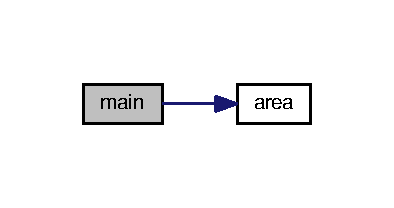
\includegraphics[width=189pt]{Slicker_8cpp_a3c04138a5bfe5d72780bb7e82a18e627_cgraph}
\end{center}
\end{figure}




\subsection{Variable Documentation}
\index{Slicker.\+cpp@{Slicker.\+cpp}!E\+P\+S\+I\+L\+ON@{E\+P\+S\+I\+L\+ON}}
\index{E\+P\+S\+I\+L\+ON@{E\+P\+S\+I\+L\+ON}!Slicker.\+cpp@{Slicker.\+cpp}}
\subsubsection[{\texorpdfstring{E\+P\+S\+I\+L\+ON}{EPSILON}}]{\setlength{\rightskip}{0pt plus 5cm}double E\+P\+S\+I\+L\+ON = 0.\+000001}\hypertarget{Slicker_8cpp_a3644fc584736c1c2e36037a085c416b9}{}\label{Slicker_8cpp_a3644fc584736c1c2e36037a085c416b9}
\index{Slicker.\+cpp@{Slicker.\+cpp}!M\+A\+X\+P\+O\+LY@{M\+A\+X\+P\+O\+LY}}
\index{M\+A\+X\+P\+O\+LY@{M\+A\+X\+P\+O\+LY}!Slicker.\+cpp@{Slicker.\+cpp}}
\subsubsection[{\texorpdfstring{M\+A\+X\+P\+O\+LY}{MAXPOLY}}]{\setlength{\rightskip}{0pt plus 5cm}const int M\+A\+X\+P\+O\+LY = 200}\hypertarget{Slicker_8cpp_ae936b8f2104cec7519d956be29b10e2b}{}\label{Slicker_8cpp_ae936b8f2104cec7519d956be29b10e2b}

%--- End generated contents ---

% Index
\backmatter
\newpage
\phantomsection
\clearemptydoublepage
\addcontentsline{toc}{chapter}{Index}
\printindex

\end{document}
